%!TEX program = xelatex
%%%%%%%%%%%%%%%%%%%%%%%这是导言部分的开始%%%%%%%%

%========= 导言部分声明文档的类型=================
\documentclass{article}

%=========导言部分可可以加载宏包=================
\usepackage{amsmath}                % 数学公式排版宏包
\usepackage{amssymb}                % 数学符号命令宏包
\usepackage{amsthm}                 % 数学定理宏包
\usepackage[UTF8]{ctex}             % 中文输入宏包
\usepackage[a4paper]{geometry}      % 页面设置宏包
\usepackage{setspace}               % 行间距宏包
\usepackage{graphicx}               % 图片宏包
\usepackage{listings}               % 代码宏包
\usepackage{color}
\usepackage{xcolor}                 % 颜色处理宏包
\usepackage{float}                  % 浮动对象式样宏包
\usepackage{fontspec}

%=========页面设置==============================
\geometry{left=1cm,right=1cm,top=1cm,bottom=2cm}
\onehalfspacing
\setlength\parindent{0em}

%=========代码格式设置============================
\definecolor{dkgreen}{rgb}{0,0.6,0}
\definecolor{gray}{rgb}{0.5,0.5,0.5}
\definecolor{mauve}{rgb}{0.58,0,0.82}
\setmonofont{Consolas}
\lstset{
	numbers = left, 	
    numberstyle = \color{gray}, 
    keywordstyle = \color{blue},
	commentstyle = \color{dkgreen}, 
	stringstyle = \color{mauve},
	basicstyle = \ttfamily,
	breaklines = true,
    frame = shadowbox, % 阴影效果
    rulesepcolor = \color{ red!20!green!20!blue!20} ,
    escapeinside = ``, % 英文分号中可写入中文
    xleftmargin = 2em,xrightmargin=2em, aboveskip=1em,
    framexleftmargin = 2em
} 

%=========导言部分可以定义标题信息===============
\title{组会报告}
\author{徐益}
\date{2018/4/26}

%%%%%%%%%%%%%%%%%%%%%%%这是导言部分的结束%%%%%%%%%

%%%%%%%%%%%%%%%%%%%%%%%这是正文部分的开始%%%%%%%%%
\begin{document}

%=========生成标题================================
\maketitle

%=========开始正文的输入==========================

%===========第一节=================
\section{本周学习内容}

1. 《多核应用编程实战》1-5章

2. LTE数据处理多核版本阅读源码

%===========第一节=================
\section{《多核应用编程实战》}
\subsection{多线程的特点}
\subsubsection{时序特点}
\begin{figure}[H]
	\centering
	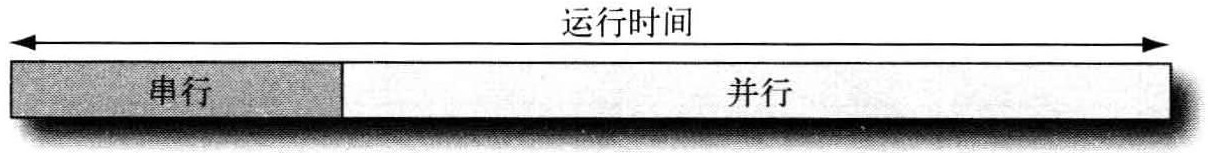
\includegraphics[width = .8\textwidth]{single_time.jpg}
	\caption{单线程时序特点}
\end{figure}
\begin{figure}[H]
	\centering
	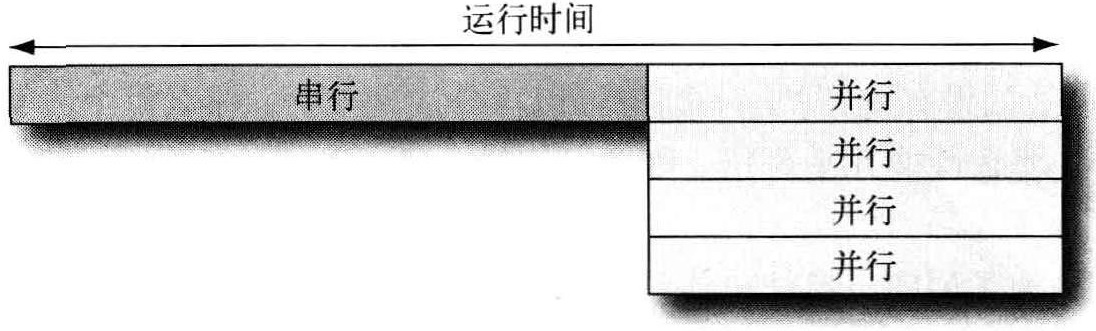
\includegraphics[width = .8\textwidth]{muti_time.jpg}
	\caption{多线程时序特点}
\end{figure}
\subsubsection{内存空间上的特点}
\begin{figure}[H]
	\centering
	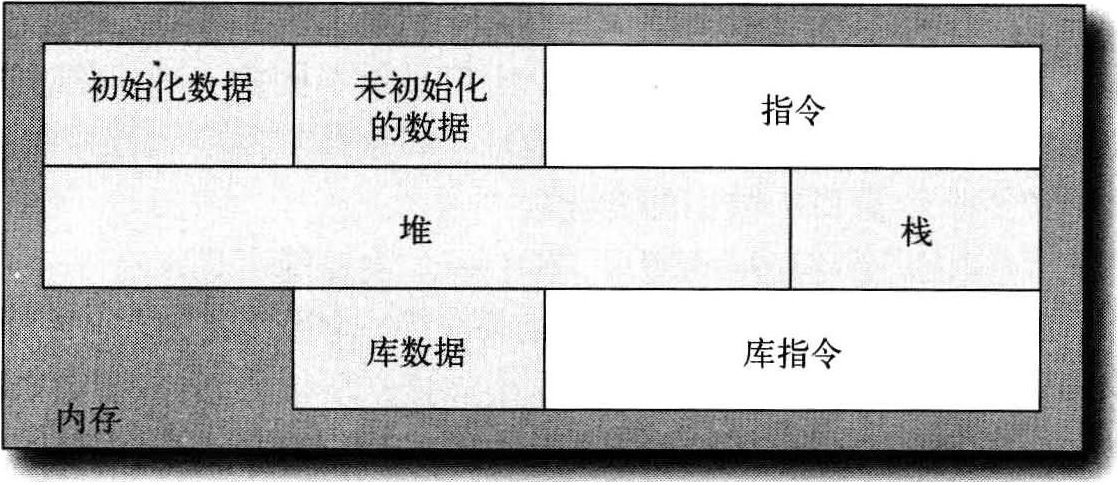
\includegraphics[width = .8\textwidth]{single_mem.jpg}
	\caption{单线程内存空间特点}
\end{figure}
\begin{figure}[H]
	\centering
	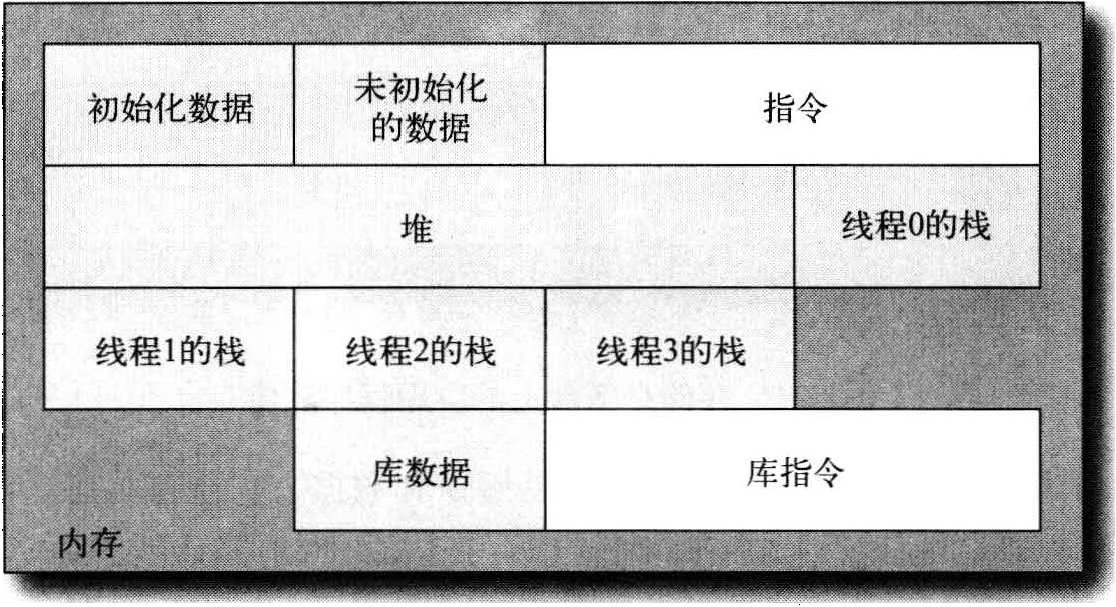
\includegraphics[width = .8\textwidth]{muti_mem.jpg}
	\caption{多线程内存空间特点}
\end{figure}

\subsection{同步与数据共享相关原语}
\begin{tabular}[H]{|l|l|}% 通过添加 | 来表示是否需要绘制竖线
	\hline  % 在表格最上方绘制横线
	原语	&	含义\\
	\hline
	互斥量   & 相互排斥的锁,一次只有一个线程获得互斥锁,从而保证对变量的访问                 \\
	\hline
	临界区   & 获取和释放互斥锁之间的代码区域                                                 \\
	\hline
	自旋锁   & 本质上是互斥锁,等待获取自旋锁的线程会不断尝试,等待获取互斥锁的线程会进入休眠 \\
	\hline
	信号量   & 可递增或递减的计数器,用于对资源存在有限限制的情况                             \\
	\hline
	读写锁   & 解决修改共享数据时的数据争用问题                                               \\
	\hline
	屏障     & 令各线程等待直到所有线程完成                                                   \\
	\hline
	条件变量 & 线程间用于沟通准备情况的变量,条件为真时唤醒线程                               \\
	\hline  % 在表格最下方绘制横线
\end{tabular}

\subsection{POSIX线程函数}
\subsubsection{基本函数}
\begin{tabular}[H]{|l|l|}% 通过添加 | 来表示是否需要绘制竖线
	\hline  % 在表格最上方绘制横线	
	函数                     & 功能\\
	\hline
	pthread\_create()        & 创建新线程\\
	\hline
	pthread\_exit()          & 主线程等待所有子线程终止后退出         \\
	\hline
	pthread\_join()          & 待线程结束,回收线程,获得返回值       \\
	\hline
	pthread\_detch()         & 使线程分离(无需等待主线程回收返回值) \\
	\hline
	pthread\_attr\_init()    & 初始化pthread属性结构                  \\
	\hline
	pthread\_attr\_destroy() & 销毁pthread属性结构                    \\
	\hline  % 在表格最下方绘制横线
\end{tabular}

\subsubsection{原语相关函数}
\begin{tabular}[H]{|l|l|}% 通过添加 | 来表示是否需要绘制竖线
	\hline  % 在表格最上方绘制横线
	函数                        & 功能                                                  \\
	\hline
	pthread\_mutex\_init()      & 互斥锁初始化                                          \\
	\hline
	pthread\_mutex\_destroy()   & 互斥锁销毁                                            \\
	\hline
	pthread\_mutex\_lock()      & 获取互斥锁                                            \\
	\hline
	pthread\_mutex\_unlock()    & 释放互斥锁                                            \\
	\hline
	pthread\_spin\_init()       & 自旋锁初始化                                          \\
	\hline
	pthread\_spin\_destroy()    & 自旋锁销毁                                            \\
	\hline
	pthread\_spin\_lock()       & 获取自旋锁                                            \\
	\hline
	pthread\_spin\_unlock()     & 释放自旋锁                                            \\
	\hline
	pthread\_rwlock\_init()     & 读写锁初始化                                          \\
	\hline
	pthread\_rwlock\_destroy()  & 读写锁销毁                                            \\
	\hline
	pthread\_rwlock\_rdlock()   & 获取读锁                                              \\
	\hline
	pthread\_rwlock\_rdunlock() & 释放读锁                                              \\
	\hline
	pthread\_rwlock\_wrlock()   & 获取写锁                                              \\
	\hline
	pthread\_rwlock\_wrunlock() & 释放写锁                                              \\
	\hline
	pthread\_barrier\_init()    & 屏障初始化                                            \\
	\hline
	pthread\_barrier\_destroy() & 屏障销毁                                              \\
	\hline
	pthread\_barrier\_wait()    & 在到达屏障的线程达到一定数量后返回                    \\
	\hline
	sem\_init()                 & 信号量初始化                                          \\
	\hline
	sem\_destroy()              & 信号量销毁                                            \\
	\hline
	sem\_open()                 & 打开命名信号量                                        \\
	\hline
	sem\_close()                & 关闭命名信号量                                        \\
	\hline
	sem\_unlink()               & 删除命名信号量                                        \\
	\hline
	sem\_wait()                 & 尝试减少非命名信号量,信号量为0时等待,直到非零时返回 \\
	\hline
	sem\_post()                 & 增加非命名信号量                                      \\
	\hline
	pthread\_cond\_init()       & 条件变量初始化                                        \\
	\hline
	pthread\_cond\_destroy()    & 条件变量销毁                                          \\
	\hline
	pthread\_cond\_signal()     & 产生唤醒信号                                          \\
	\hline
	pthread\_cond\_broadcast()  & 广播唤醒信号                                          \\
	\hline
	pthread\_cond\_wait()       & 等待唤醒信号                                          \\
	\hline  % 在表格最下方绘制横线
\end{tabular}

%===========第二节=================
\section{LTE数据处理多线程版本源码}
\subsection{thread\_pool.h}
\subsubsection{void pool\_init(int coreId\_start, int \_threadNum, int pool\_index);}
\textbf{功能:}初始化线程池\\
\textbf{参数:}\\
\begin{tabular}[H]{|l|l|}% 通过添加 | 来表示是否需要绘制竖线
	\hline  % 在表格最上方绘制横线
	参数              & 含义             \\
	\hline
	int coreId\_start & 线程初始序号     \\
	\hline
	int threadNum     & 线程池中线程数目 \\
	\hline
	int pool\_index   & 线程池序号       \\
	\hline
\end{tabular}

\subsubsection{void pool\_add\_task(Fun myfun, void *arg, int pool\_index);}
\textbf{功能:}在线程池中添加任务\\
\textbf{参数:}\\
\begin{tabular}[H]{|l|l|}% 通过添加 | 来表示是否需要绘制竖线
	\hline  % 在表格最上方绘制横线
	参数            & 含义       \\
	\hline
	Fun myfun       & 函数名     \\
	\hline
	void *arg       & 函数参数   \\
	\hline
	int pool\_index & 线程池序号 \\
	\hline
\end{tabular}

\subsubsection{void pool\_destroy(int pool\_index);}
\textbf{功能:}待所有线程完成后销毁线程及线程池\\
\textbf{参数:}\\
\begin{tabular}[H]{|l|l|}% 通过添加 | 来表示是否需要绘制竖线
	\hline  % 在表格最上方绘制横线
	参数            & 含义       \\
	\hline
	int pool\_index & 线程池序号 \\
	\hline
\end{tabular}

\subsection{main.c}

\lstset{language=C++}
\begin{lstlisting}
const int threadNum_tx = 1;		// 发送端线程数
const int threadNum_rx = 1;		// 接收端线程数

/* 声明互斥锁 */
pthread_mutex_t mutex1_tx;		// crc_cbsegm中的互斥锁
pthread_mutex_t mutex2_tx;		// crc_mod中的互斥锁
pthread_mutex_t mutex1_rx;		// chest_calsym中的互斥锁
pthread_mutex_t mutex2_rx;		// derm_crc中的互斥锁
pthread_mutex_t mutex3_rx;		// crc_check中的互斥锁

/* 声明信号量 */
sem_t exit_signal;			// 收发端主线程完成数信号量
//test
sem_t tx_signal;			// 开启发送端主线程的信号量
sem_t rx_signal;			// 开启接收端主线程的信号量

int main(){
	
	/* 初始化互斥锁 */
	pthread_mutex_init(&mutex1_tx,NULL);
	pthread_mutex_init(&mutex2_tx,NULL);
	pthread_mutex_init(&mutex1_rx,NULL);
	pthread_mutex_init(&mutex2_rx,NULL);
	pthread_mutex_init(&mutex3_rx,NULL);
	
	/* 初始化信号量 */
	sem_init(&exit_signal,0,0);
	sem_init(&tx_signal,0,0);
	sem_init(&rx_signal,0,0);
	
	/* 初始化线程池 */
	pool_init(0, 1, 0);				// 发送端主线程池
	printf("creat pool 0...\n");
	pool_init(1, 1, 1);				// 接收端主线程池
	printf("creat pool 1...\n");
	pool_init(2, threadNum_tx, 2);			// 发送端任务线程池
	printf("creat pool 2...\n");
	pool_init(2 + threadNum_tx, threadNum_rx, 3);	// 接收端任务线程池
	printf("creat pool 3...\n");
	
	/* 添加发送端主任务 */
	pool_add_task(TaskScheduler_tx, NULL, 0);
	printf("add tx taskScheduler to pool 0...\n");
	/* 添加接收端主任务 */
	pool_add_task(TaskScheduler_rx, NULL, 1);
	printf("add rx taskScheduler to pool 1...\n");

	/* 等待收发机主任务完成 */
	for(int i = 0; i < 2; i++) sem_wait(&exit_signal);

	/* 销毁线程池 */
	pool_destroy(0);
	pool_destroy(1);

	/* 销毁信号量*/
	sem_destroy(&exit_signal);

	return 0;
}
\end{lstlisting}

\subsection{收发主线程流程}
\begin{figure}[H]
	\centering
	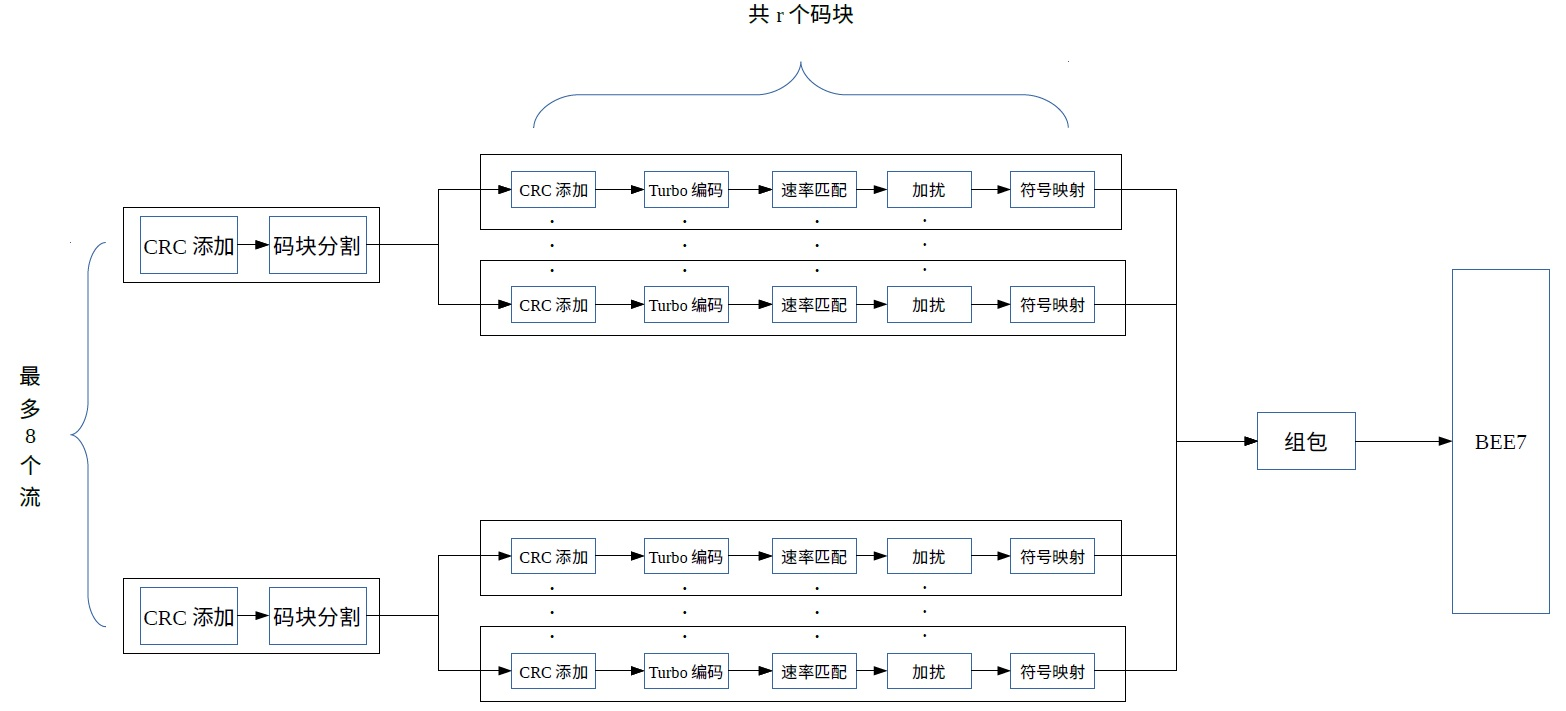
\includegraphics[width = \textwidth]{flow_muti_tx.jpg}
	\caption{发送端主线程流程图}
\end{figure}
\begin{figure}[H]
	\centering
	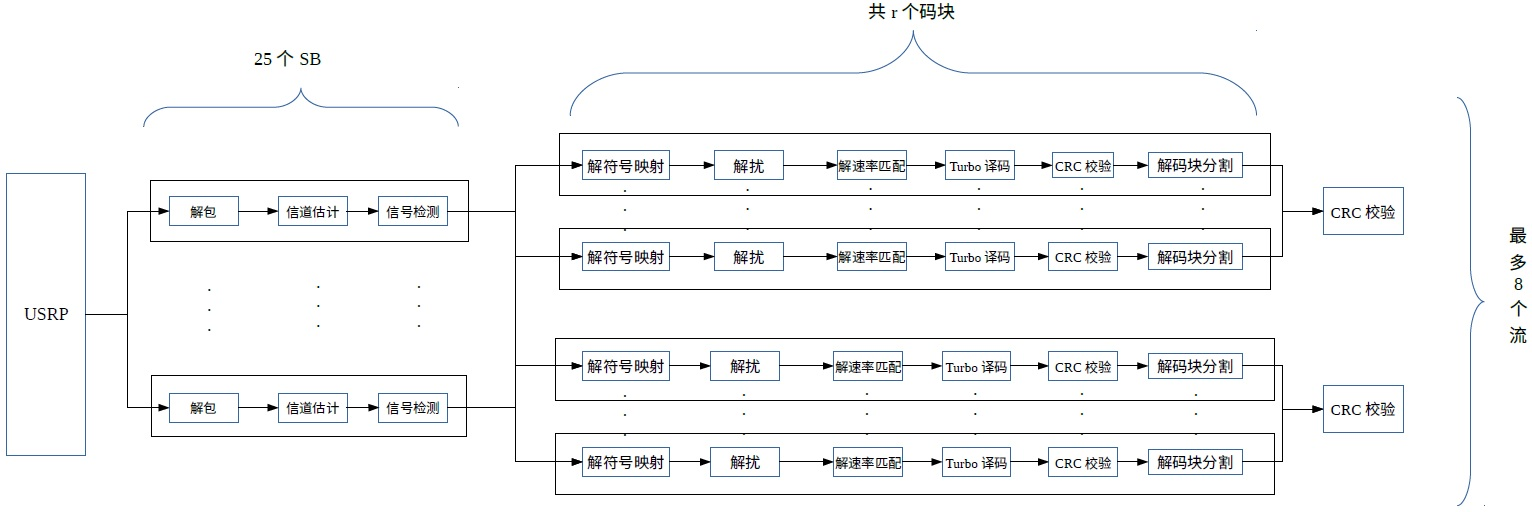
\includegraphics[width = \textwidth]{flow_muti_rx.jpg}
	\caption{接收端主线程流程图}
\end{figure}

%===========存在问题=================
\section{存在问题}
1. 每个收发主线程处理多少数据?一帧?分成八个流?

2. 为什么这样分割收发端主线程?是否越细分越好?

3. 收发端分离后通信的具体方式?DPDK?

%===========下周计划=================
\section{下周计划}
1. 继续阅读多线程部分源码

2. 学习DPDK

\end{document}
%%%%%%%%%%%%%%%%%%%%%%%这是正文部分的结束%%%%%%%%%%%%
